\chapter{Mikrobiom dan Simbiosis}\label{ch:b3:microbiomes}

Anda mengusung sekitar tiga puluh delapan triliun bakteri, kira-kira satu bagi
tiap sel Anda sendiri, kebanyakan di dalam semeter terakhir usus Anda, tempat
bobotnya kurang lebih sebobot otak Anda dan gennya seratus kali lebih banyak
daripada gen Anda. Seekor mencit yang dibesarkan tanpa satu pun di antaranya
memerlukan sepertiga lebih banyak makanan untuk menjaga bobotnya, sistem
imunnya kerdil, dan tingkahnya aneh. Sebatang kacang memberi sepersepuluh
gulanya kepada bakteri di dalam bintil pada akarnya lalu memperoleh nitrogennya
sebagai balasan; empat perlima seluruh tumbuhan darat menukar gula dengan
fosfat bersama jamur yang membungkus akarnya, sebagaimana telah mereka lakukan
selama empat ratus juta tahun; sebuah karang adalah hewan yang beternak alga di
dalam selnya lalu mati ketika lautnya cukup menghangat untuk membuatnya
mengusir alga itu. Makhluk hidup bukanlah perseorangan melainkan persekutuan,
dan bab ini memperlakukan biologi kemitraannya: bagaimana kemitraan itu dicacah
dan dicirikan dengan pengurutan, apa yang dipertukarkan para mitra, bagaimana
pertukarannya dirundingkan dan diawasi, serta mengapa sebagian mitra berakhir
sebagai organel.

\section{Kata bagi hidup bersama}

\begin{definition}[Simbiosis]\label{def:b3:microbiomes:symbiosis}
\index{simbiosis}\index{mutualisme}\index{komensalisme}%
\index{holobion}\index{mikrobiom}\index{penularan menegak}
\emph{Simbiosis} adalah perkaitan yang lestari dan akrab antara jasad dari
spesies yang berbeda; ia sebuah \emph{mutualisme} bila keduanya beroleh
untung, sebuah \emph{komensalisme} bila satu beroleh untung dan yang lain tidak
terpengaruh, dan sebuah parasitisme bila satu beroleh untung dengan mengorbankan
yang lain --- dan pasangan yang sama dapat bergerak sepanjang garis itu menurut
keadaan. Sebuah \emph{endosimbion} hidup di dalam sel inangnya; mitra yang
\emph{obligat} tidak dapat hidup sendirian. Simbion ditularkan secara
\emph{menegak}, dari induk ke keturunan (\emph{Buchnera} kutu daun lewat
telurnya), atau secara \emph{mendatar}, yang diperoleh baru tiap angkatan dari
lingkungan atau dari inang lain (\emph{Vibrio} cumi-cumi, bakteri usus manusia).
\emph{Mikrobiom} adalah seluruh masyarakat mikroba sebuah habitat --- sebuah
usus, sebuah permukaan daun, segram tanah --- dan \emph{holobion} adalah inang
bersama mikrobiomnya, yang dipandang sebagai satuan yang dilihat seleksi alam.
\end{definition}

\begin{example}[Tiga mitra obligat]\label{ex:b3:microbiomes:obligate}
\emph{Buchnera} kutu daun telah hidup di dalam sel inangnya selama dua ratus
juta tahun, membuat asam amino esensial yang tidak ada pada getah floem, dan
telah menyusutkan genomnya menjadi \qty{640}{kb} --- sepertujuh genom kerabatnya
yang hidup bebas --- dengan kehilangan tiap gen yang kini dipasok inangnya.
Bakteri \emph{Wolbachia}, yang ada pada dua pertiga spesies serangga,
ditularkan lewat telur saja, sehingga ia berevolusi untuk memihak betina: ia
membunuh embrio jantan, membetinakannya, atau membuat telur betina yang tidak
terinfeksi mati ketika dibuahi jantan yang terinfeksi (\emph{ketaksesuaian
sitoplasma}), yang menyebarkannya ke seluruh populasi; nyamuk yang
mengusungnya buruk menularkan demam berdarah, dan melepasnya telah memangkas
demam berdarah di beberapa kota. Amoeba \emph{Paulinella} memasukkan sebuah
sianobakteri sekitar seratus juta tahun lalu yang kini bukan lagi betul-betul
bakteri maupun betul-betul kloroplas --- sebuah asal usul organel fotosintesis
yang kedua dan mandiri, yang tertangkap di tengah jalan.
\end{example}

\section{Mencacah sebuah masyarakat}

\begin{method}[Memerikan sebuah mikrobiom dengan pengurutan]\label{met:b3:microbiomes:16s}
\index{pengurutan rRNA 16S}\index{metagenomika}%
\index{satuan taksonomi operasional}
Kebanyakan mikroba tidak dapat dibiakkan; mereka dicacah lewat DNA-nya. (1)
Petiklah DNA dari contohnya --- tinja, tanah, air laut yang disaring ke sebuah
selaput. (2) Entah lipatgandakan gen bagi RNA ribosom subunit kecil
(\emph{16S}) dengan pemula yang cocok dengan daerah semestanya, lalu urutkan
daerah berubah-ubah di antaranya --- sebuah survei \emph{amplikon}, yang murah,
yang mengenali bakteri sampai kira-kira marganya lalu mencacahnya lewat cacah
\omterm{def:b3:genomics:ngs}{bacaan}; atau urutkan seluruh DNA-nya --- \emph{metagenomika senapan}, yang
memulihkan gen dan genom utuh sehingga melaporkan apa yang dapat dilakukan
masyarakat itu, bukan hanya siapa yang ada di sana. (3) Gugusilah \omterm{def:b3:genomics:ngs}{bacaannya}
menjadi ragam urutan atau \emph{\omterm{met:b3:microbiomes:16s}{satuan taksonomi operasional}} (OTU, lazimnya
pada keserupaan \qty{97}{\%} bagi sebuah ``spesies''), tetapkanlah
kedudukannya dengan membandingkannya dengan pangkalan data
(\cref{ch:b3:bioinformatics}), lalu tabelkanlah cacahnya tiap contoh. (4)
Hitunglah keanekaan di dalam sebuah contoh lalu bandingkanlah susunannya
antarcontoh. Cacahnya nisbi --- \omterm{def:b3:genomics:ngs}{bacaan} sebuah contoh berjumlah sebuah total
tetap --- dan berat sebelah karena pemetikan, pemula, dan cacah salinan,
sehingga perbedaan antarcontoh yang diolah dengan cara yang sama terpercaya
padahal angka mutlaknya tidak.
\end{method}

\begin{definition}[Keanekaan]\label{def:b3:microbiomes:diversity}
\index{kekayaan spesies}\index{indeks Shannon}%
\index{indeks Simpson}\index{penjarangan}
Bagi sebuah masyarakat beranggota $S$ spesies dengan kelimpahan nisbi $p_{1},\dots,
p_{S}$ ($\sum p_{i} = 1$): \emph{kekayaannya} adalah $S$; \emph{indeks
Shannon} $H = -\sum_{i} p_{i}\ln p_{i}$ mengukur ketakpastian tentang spesies
sebuah individu yang ditarik secara acak, dan $e^{H}$ adalah cacah spesies
yang sama melimpahnya yang akan memberikan ketakpastian yang sama (yakni cacah
spesies yang mujarab); \emph{indeks Simpson} $D = \sum_{i} p_{i}^{2}$ adalah
peluang bahwa dua individu yang ditarik secara acak berspesies sama, dan $1/D$
adalah cacah mujarab yang lain, yang berbobot ke arah spesies yang lazim.
Kekayaannya bergantung pada berapa banyak individu yang telah dilihat: sebuah
\emph{kurva penjarangan} memetakan spesies yang ditemukan terhadap cacah
individu yang dicontoh, lalu mendatar ketika kebanyakan spesiesnya telah
terlihat.
\end{definition}

\begin{theorem}[Penjarangan]\label{thm:b3:microbiomes:rarefaction}
\index{penjarangan!rumus}\index{cakupan Good}
Sebuah contoh berisi $N$ individu dari $S$ spesies, dengan $N_{i}$ individu
berspesies $i$. Harapan cacah spesies di dalam sebuah anak contoh acak
beranggota $n$ individu, yang ditarik tanpa pengembalian, adalah
\[
E[S_{n}] = \sum_{i=1}^{S}\left[1 - \frac{\binom{N - N_{i}}{n}}
{\binom{N}{n}}\right],
\]
yang naik seiring $n$ lalu sama dengan $S$ pada $n = N$. Dua contoh yang
berlainan ukurannya dibandingkan dengan menjarangkan keduanya ke $n$ yang sama.
Bagian individu masyarakat itu yang tergolong spesies yang belum terlihat
ditaksir dengan \emph{\omterm{thm:b3:microbiomes:rarefaction}{cakupan Good}}: kira-kira $f_{1}/N$, dengan
$f_{1}$ cacah spesies yang terlihat tepat sekali (tunggalan).
\end{theorem}
\begin{proof}
Spesies $i$ tidak ada di dalam anak contohnya tepat ketika semua $n$
individunya ditarik dari $N - N_{i}$ yang lain, yang terjadi pada
$\binom{N - N_{i}}{n}$ dari $\binom{N}{n}$ anak contoh yang sama peluangnya;
jadi spesies $i$ hadir dengan peluang $1 - \binom{N-N_{i}}{n}/
\binom{N}{n}$, dan harapan cacah spesies yang hadir adalah jumlah
peluang itu (harapan sebuah jumlah penunjuk). Tiap sukunya
naik seiring $n$, dan pada $n = N$ tiap binomial pada pembilangnya
nol. Taksiran Good: sebuah individu yang ditarik berikutnya tergolong spesies
yang belum terlihat kira-kira dengan peluang bahwa sebuah individu contoh yang
dipilih secara acak adalah satu-satunya dari jenisnya, yakni $f_{1}/N$ (Good,
1953); pembenarannya diakui saja di sini.
\end{proof}

\begin{example}[Dua usus]\label{ex:b3:microbiomes:two-guts}
Sebuah contoh $1000$ \omterm{def:b3:genomics:ngs}{bacaan} dari seseorang menghasilkan $150$ spesies, dengan
$H = 3.5$ dan $40$ tunggalan; sebuah contoh $5000$ \omterm{def:b3:genomics:ngs}{bacaan} dari orang lain
menghasilkan $260$ spesies. Yang kedua belum tentu lebih beraneka: ia
dicontoh lima kali lebih dalam, dan menjarangkannya ke $1000$ \omterm{def:b3:genomics:ngs}{bacaan}
mungkin memberi $150$ juga. Cakupan contoh yang pertama adalah $1 - 40/1000 =
\qty{96}{\%}$: empat persen bakteri di dalam usus itu tergolong
spesies yang tidak pernah dilihat contohnya, dan contoh yang lebih dalam akan
menemukannya. Cacah mujarabnya, yakni kerataan senilai $e^{3.5} \approx 33$
spesies terhadap kekayaan $150$, mengatakan bahwa beberapa spesies menguasainya
--- dan begitulah rupa tiap usus.
\end{example}

\begin{omfigure}
\begin{tikzpicture}
\begin{axis}[
  width=0.68\linewidth, height=5.6cm,
  axis x line=bottom, axis y line=left,
  xmin=0, xmax=5000, ymin=0, ymax=300,
  xlabel={bacaan yang dicontoh, $n$}, ylabel={spesies yang teramati},
  xlabel style={font=\small, at={(axis description cs:0.5,-0.12)}, anchor=north}, ylabel style={font=\small},
  tick label style={font=\small}, xtick={0,1000,2000,3000,4000,5000}, ytick={0,100,150,200,260},
  clip=false,
]
\addplot[very thick, omDef, domain=0:5000, samples=60] {260*(1-exp(-x/1500))};
\addplot[very thick, omThm, domain=0:1000, samples=30] {150*(1-exp(-x/300))*1.0};
\addplot[very thick, omThm, dashed, domain=1000:5000, samples=30] {150*(1-exp(-x/300))*1.0 + 8*(1-exp(-(x-1000)/2000))};
\draw[dashed, gray] (axis cs:1000,0) -- (axis cs:1000,300);
\node[font=\scriptsize, omDef, anchor=north west] at (axis cs:1200,292) {usus kedua: $260$ spesies pada $5000$ bacaan};
\node[font=\scriptsize, omThm, anchor=north east] at (axis cs:4900,140) {usus pertama: $150$ pada $1000$, hampir datar};
\node[font=\scriptsize, gray, anchor=south west] at (axis cs:1050,10) {jarangkan di sini untuk membandingkan};
\end{axis}
\end{tikzpicture}

{\small Kurva \omterm{def:b3:microbiomes:diversity}{penjarangan}. Spesies yang ditemukan naik seiring \omterm{def:b3:genomics:ngs}{bacaan} yang
dicontoh lalu mendatar ketika masyarakatnya terkuras; dua contoh dibandingkan
pada kedalaman yang sama. Di sini usus kedua masih mendaki pada $5000$ \omterm{def:b3:genomics:ngs}{bacaan},
sehingga kekayaan sejatinya lebih tinggi lagi.}
\end{omfigure}

\section{Mikrobiom manusia}

\begin{definition}[Masyarakat usus]\label{def:b3:microbiomes:gut}
\index{mikrobiom usus}\index{asam lemak rantai pendek}%
\index{ketahanan penjajahan}\index{disbiosis}
Usus manusia memuat sekitar $4\times 10^{13}$ bakteri, hampir semuanya di dalam
kolon pada $10^{11}$ per gram isi, terhadap $10^{3}$ per gram di dalam
lambung yang asam dan $10^{4}$--$10^{7}$ sepanjang usus halus, yang
aliranya cepat dan empedunya bermusuhan. Sekitar lima ratus sampai seribu
spesies tiap orang, kebanyakan dari dua filum, yakni Bacteroidetes dan
Firmicutes, hampir semuanya anaerob; himpunan tiap orang berbeda dan
mantap bertahun-tahun, yang sebagian besar dipancangkan pada tiga tahun pertama
kehidupan dari ibunya dan rumah tangganya. Apa yang mereka lakukan: meragikan
serat yang tidak dapat dicerna enzim manusia menjadi \emph{asam lemak rantai
pendek} --- asetat, propionat, butirat --- yang memberi makan sel kolon sendiri
lalu memasok sampai sepersepuluh kalori inangnya; membuat vitamin~K dan
beberapa vitamin B; mengubah asam empedu dan obat; menempati tiap ceruk
sehingga seorang penyerbu tidak menemukan pijakan (\emph{ketahanan
penjajahan}); serta melatih sistem imun, yang sel~T pengaturnya dan sel
penyekresi IgA-nya berkembang sebagai tanggapan terhadapnya
(\cref{ch:b3:adaptive-immunity}). Sebuah masyarakat yang bergeser dari keadaan
ini --- lebih sedikit spesies, lebih sedikit peragi, lebih banyak aerob
fakultatif --- adalah sebuah \emph{disbiosis}, yang terlihat pada penyakit
radang usus, sesudah \omterm{def:b3:bacteriology:antibiotics}{antibiotik}, dan pada kegemukan, meskipun mana yang sebab
dan mana yang akibat biasanya tidak jelas.
\end{definition}

\begin{proof}[Bukti eksperimental]
Mencit yang dibesarkan bebas kuman di dalam pengasing steril (Gordon dan
rekannya, dasawarsa 2000-an) berdinding usus tipis, berorgan limfoid kecil,
berkadar antibodi rendah, dan memerlukan \qty{30}{\%} lebih banyak kalori untuk
menjaga bobotnya; ketika dijajahi mikrobiota mencit normal, mereka bertambah
lemak dalam dua minggu. Ketika diberi mikrobiota mencit gemuk alih-alih mencit
kurus, mencit bebas kuman bertambah lebih banyak lemak pada makanan yang sama
(Turnbaugh, 2006): masyarakatnya sendirilah yang memengaruhi panenan tenaga.
Pada manusia, kolitis \emph{Clostridioides difficile} yang berulang --- sebuah
\omterm{def:b3:microbiomes:gut}{disbiosis} yang di dalamnya \omterm{def:b3:bacteriology:antibiotics}{antibiotik} telah membersihkan pesaing sebuah
pembentuk spora penghasil racun --- disembuhkan pada \qty{94}{\%} pasien dengan
pemasukan tinja seorang donor yang sehat, terhadap \qty{31}{\%} dengan
\omterm{def:b3:bacteriology:antibiotics}{antibiotik} baku (van~Nood, 2013), yakni uji acak pertama yang di dalamnya
sebuah masyarakat, bukan sebuah molekul, menjadi obatnya.
\end{proof}

\begin{omfigure}
\begin{tikzpicture}
\begin{axis}[
  width=0.68\linewidth, height=5.4cm,
  ybar, bar width=18pt,
  axis x line=bottom, axis y line=left,
  ymode=log, ymin=1, ymax=1e13,
  symbolic x coords={lambung, duodenum, jejunum, ileum, kolon},
  xtick=data, ytick={1e1,1e3,1e5,1e7,1e9,1e11},
  ylabel={bakteri per gram isi},
  ylabel style={font=\small}, tick label style={font=\small},
  clip=false,
]
\addplot[fill=omDef!40, draw=omDef] coordinates {(lambung,1e3) (duodenum,1e4) (jejunum,1e5) (ileum,1e7) (kolon,1e11)};
\node[font=\scriptsize, anchor=west, xshift=10pt] at (axis cs:lambung,3e3) {asam, pH 2};
\node[font=\scriptsize, anchor=south] at (axis cs:jejunum,1.5e5) {empedu, aliran cepat};
\node[font=\scriptsize, anchor=south, align=center] at (axis cs:kolon,1.5e11) {lambat dan anaerob:\\sang peragi};
\end{axis}
\end{tikzpicture}

{\small Kerapatan bakteri sepanjang usus manusia, pada skala logaritma:
sebuah kenaikan seratus juta kali lipat dari lambung yang asam ke kolon,
tempat hampir seluruh mikroba tubuh hidup.}
\end{omfigure}

\begin{omfigure}
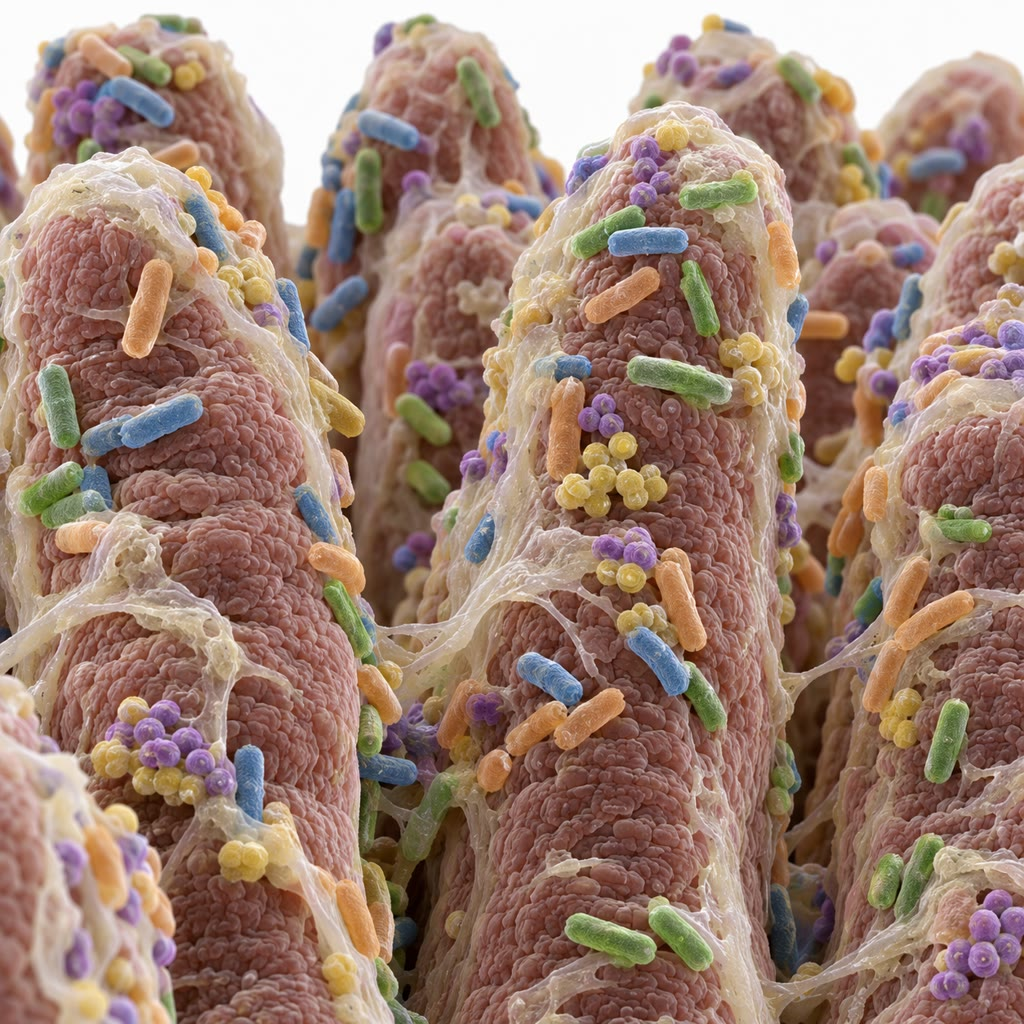
\includegraphics[width=0.40\linewidth]{images/book5/ai/b5-14-gut-microbiota.jpg}

{\small Permukaan lapisan usus di bawah mikroskop elektron payar, dengan
bakteri beberapa jenis bersarang di dalam lendir di antara
jonjot usus.}
\end{omfigure}

\section{Tumbuhan dan mitranya}

\begin{definition}[Simbiosis kacang--rizobium]\label{def:b3:microbiomes:nodule}
\index{rizobia}\index{bintil akar}\index{faktor Nod}%
\index{leghemoglobin}\index{nitrogenase}
Kacang-kacangan merumahkan bakteri pemfiksasi nitrogen (\emph{rizobia}) di
dalam \emph{bintil akar}, yakni organ yang dibangun untuk tujuan itu sesudah
sebuah dialog molekuler. Akarnya menyekresikan flavonoid; sebuah rizobium dari
spesies yang cocok menjawab dengan \emph{faktor Nod} ---
lipokitooligosakarida yang hiasannya menentukan mitranya; sebuah kinase
reseptor pada rambut akar mengikatnya lalu memicu ayunan kalsium di dalam inti,
melingkarnya rambut akar di sekeliling bakterinya, serta sebuah \emph{benang
infeksi} yang tumbuh ke dalam menembus sel sementara korteks di bawahnya mulai
membelah menjadi sebuah bintil. Bakterinya dilepaskan ke dalam sel bintil di
dalam selaput lalu berdiferensiasi menjadi \emph{bakteroid} yang mengungkapkan
\emph{nitrogenase}, yakni enzim yang mereduksi N$_{2}$ menjadi amonia dengan
ongkos enam belas ATP tiap molekul. Nitrogenase dimusnahkan oksigen, padahal
bakteroidnya bernapas keras; bintilnya menyelesaikan pertentangan itu dengan
sebuah penghadang pembauran dan dengan \emph{leghemoglobin}, yakni sebuah
hemoglobin tumbuhan yang mengikat oksigen dengan erat lalu mengantarkannya ke
bakteroid pada kepekatan bebas yang rendah --- itulah yang membuat bintil yang
terpotong berwarna merah muda. Tumbuhannya membayar enam sampai sepuluh persen
hasil fotosintesisnya lalu menerima sebagian besar nitrogennya; nitrogen
yang difiksasi tanaman kacang sedunia mendekati nitrogen yang dibuat industri
pupuk.
\end{definition}

\begin{omfigure}
\begin{tikzpicture}[every node/.style={font=\scriptsize}, >=stealth]
  % stage 1: root hair and bacteria, flavonoid / Nod factor exchange
  \begin{scope}
    \draw[thick, omMeth!60!black, fill=omMeth!15] (0,0) rectangle (1.2,3.0);
    \draw[thick, omMeth!60!black, fill=omMeth!15] (1.2,1.6) .. controls (2.4,1.7) and (2.6,2.6) .. (2.9,2.4) .. controls (2.5,2.3) and (2.3,1.4) .. (1.2,1.2) -- cycle;
    \foreach \p in {(3.1,2.7),(3.4,2.3),(3.3,1.9)} \fill[omProp] \p ellipse (0.14 and 0.07);
    \draw[->, omMeth!60!black, thick] (2.6,1.5) -- (3.2,1.4); \node[below, omMeth!60!black] at (3.0,1.35) {flavonoid};
    \draw[<-, omProp, thick] (2.5,2.85) -- (3.0,3.0); \node[above, omProp] at (2.4,2.95) {faktor Nod};
    \node[below, align=center] at (1.6,-0.2) {1. dialog: rambut akar\\dan rizobia};
  \end{scope}
  % stage 2: curled hair, infection thread
  \begin{scope}[xshift=4.6cm]
    \draw[thick, omMeth!60!black, fill=omMeth!15] (0,0) rectangle (1.2,3.0);
    \draw[thick, omMeth!60!black, fill=omMeth!15] (1.2,1.6) .. controls (2.3,1.8) and (2.8,2.6) .. (2.2,2.8) .. controls (1.9,2.9) and (1.8,2.5) .. (2.0,2.4) .. controls (2.3,2.2) and (1.9,1.3) .. (1.2,1.2) -- cycle;
    \draw[omProp, very thick] (2.05,2.55) .. controls (1.8,2.1) and (1.4,1.7) .. (0.4,1.3);
    \foreach \p in {(1.85,2.3),(1.5,1.9),(1.1,1.6),(0.7,1.4)} \fill[omProp] \p ellipse (0.1 and 0.05);
    \node[right, omProp, font=\tiny] at (2.3,1.0) {benang infeksi};
    \foreach \p in {(0.3,0.5),(0.6,0.7),(0.9,0.5)} \draw[omMeth!60!black] \p circle (0.12);
    \node[below, align=center] at (1.6,-0.2) {2. rambut melingkar; benang masuk;\\sel korteks membelah};
  \end{scope}
  % stage 3: nodule
  \begin{scope}[xshift=9.0cm]
    \draw[thick, omMeth!60!black, fill=omMeth!15] (0,0) rectangle (1.2,3.0);
    \draw[thick, omThm!60!black, fill=omThm!25] (1.2,1.5) ellipse (1.3 and 1.0);
    \foreach \p in {(1.0,1.5),(1.5,1.8),(1.6,1.2),(1.1,1.9),(1.2,1.1),(2.0,1.5)} \fill[omProp] \p circle (0.1);
    \node[right, align=left] at (2.6,2.0) {bintil: bakteroid\\dengan nitrogenase};
    \node[right, align=left, omThm!60!black] at (2.6,1.1) {merah muda: leghemoglobin\\menjaga O$_2$ rendah};
    \draw[->, thick] (0.6,2.4) -- (1.0,2.0) node[pos=0, above] {gula};
    \draw[<-, thick] (0.6,0.6) -- (1.0,1.0) node[pos=0, below] {NH$_3$};
    \node[below, align=center] at (1.6,-0.2) {3. bakteroid memfiksasi N$_2$;\\gula ditukar amonia};
  \end{scope}
\end{tikzpicture}

{\small Membuat sebuah bintil. Flavonoid dari akarnya dan \omterm{def:b3:microbiomes:nodule}{faktor Nod} dari
rizobiumnya mengenali para mitra; rambut akarnya melingkar, sebuah benang
infeksi mengusung bakterinya ke dalam, dan korteksnya membangun sebuah bintil
yang di dalamnya bakteroid, yang dijaga tetap beroksigen rendah oleh
\omterm{def:b3:microbiomes:nodule}{leghemoglobin}, memfiksasi nitrogen untuk ditukar gula.}
\end{omfigure}

\begin{definition}[Mikoriza]\label{def:b3:microbiomes:mycorrhiza}
\index{mikoriza}\index{mikoriza arbuskular}\index{jalur simbiosis bersama}
\emph{Mikoriza} adalah perkaitan akar dengan jamur, yang ditemukan pada sekitar
\qty{80}{\%} spesies tumbuhan dan pada fosil tumbuhan darat yang terawal.
Pada \emph{mikoriza arbuskular}, jamurnya (seekor Glomeromycete) memasuki
sel akarnya lalu bercabang menjadi sebuah arbuskul serupa pohon yang
melintasinya fosfat, nitrogen, dan air lewat ke tumbuhannya serta gula dan
lipid ke jamurnya; hifa jamurnya memperluas permukaan penyerap akarnya seratus
kali lipat lalu menjangkau fosfat yang tidak terjangkau akarnya. Pada
\emph{ektomikoriza}, milik pohon hutan, jamurnya menyarungi akarnya lalu
tumbuh di antara selnya. Gen tumbuhan yang memasukkan jamurnya adalah
\emph{jalur \omterm{def:b3:microbiomes:symbiosis}{simbiosis} bersama} yang sama --- reseptor, lonjakan kalsium,
faktor transkripsi --- yang dipakai ulang kacang-kacangan bagi \omterm{def:b3:microbiomes:nodule}{rizobia}:
bintilnya adalah sebuah penemuan lanjut yang dibangun di atas kemitraan jamur
yang empat ratus juta tahun lebih tua.
\end{definition}

\begin{proposition}[Perdagangan dan pengawasannya]\label{prop:b3:microbiomes:sanctions}
\index{pemilihan mitra}\index{sanksi}\index{pencurang}
Sebuah \omterm{def:b3:microbiomes:symbiosis}{mutualisme} adalah pertukaran, dan tiap mitra terpilih untuk memberi
lebih sedikit lalu mengambil lebih banyak; ia bertahan karena mitra yang lain
dapat membalas. Kacang-kacangan membatasi oksigen bagi bintil yang \omterm{def:b3:microbiomes:nodule}{rizobianya}
tidak memfiksasi nitrogen, sehingga memotong separuh perkembangbiakannya
(Kiers, 2003): itulah \emph{sanksi}. Tumbuhan di dalam jaringan \omterm{def:b3:microbiomes:mycorrhiza}{mikoriza}
membagikan lebih banyak karbon kepada mitra jamur yang menghantarkan lebih
banyak fosfat, dan jamurnya lebih banyak fosfat kepada akar yang membayar
lebih banyak karbon --- sebuah pasar yang di dalamnya kedua pihak mengganjar
pedagang yang lebih baik (Kiers, 2011). Cumi-cumi mengusir bakteri organ cahaya
yang tidak berpendar; sistem imun manusia membiarkan komensal yang tinggal di
dalam rongga usus lalu menyerang yang menyeberangi dindingnya. Bila sebuah
inang tidak dapat memilih maupun menjatuhkan sanksi --- sebuah endosimbion yang
diwarisi lewat telur --- keselarasan kepentingannya justru datang dari nasib
bersama: sebuah simbion yang ditularkan secara menegak berkembang biak hanya
ketika inangnya berkembang biak, dan seleksi atas simbionnya memihak
perkembangbiakan inangnya. Cara penularannya dengan demikian meramalkan watak
kemitraannya: \omterm{def:b3:microbiomes:symbiosis}{penularan menegak} ke arah \omterm{def:b3:microbiomes:symbiosis}{mutualisme} dan ketergantungan,
penularan mendatar ke arah pemerasan yang dikekang pengawasan.
\end{proposition}
\admitted

\begin{omfigure}
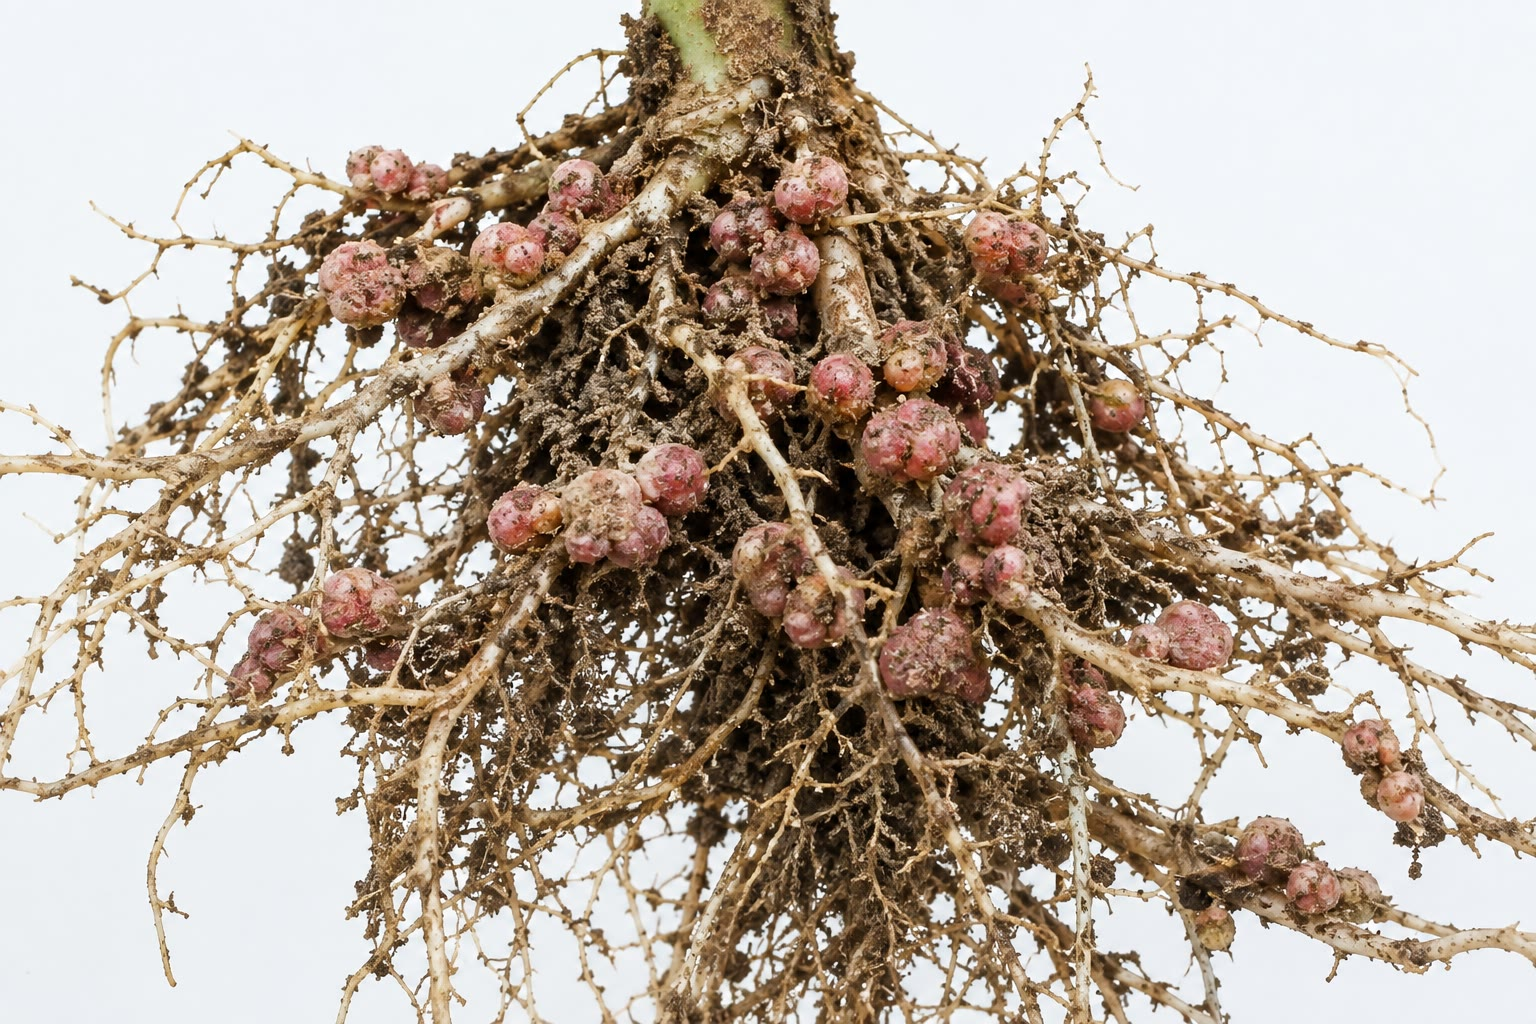
\includegraphics[width=0.46\linewidth]{images/book5/ai/b5-14-root-nodules.jpg}\hspace{0.04\linewidth}
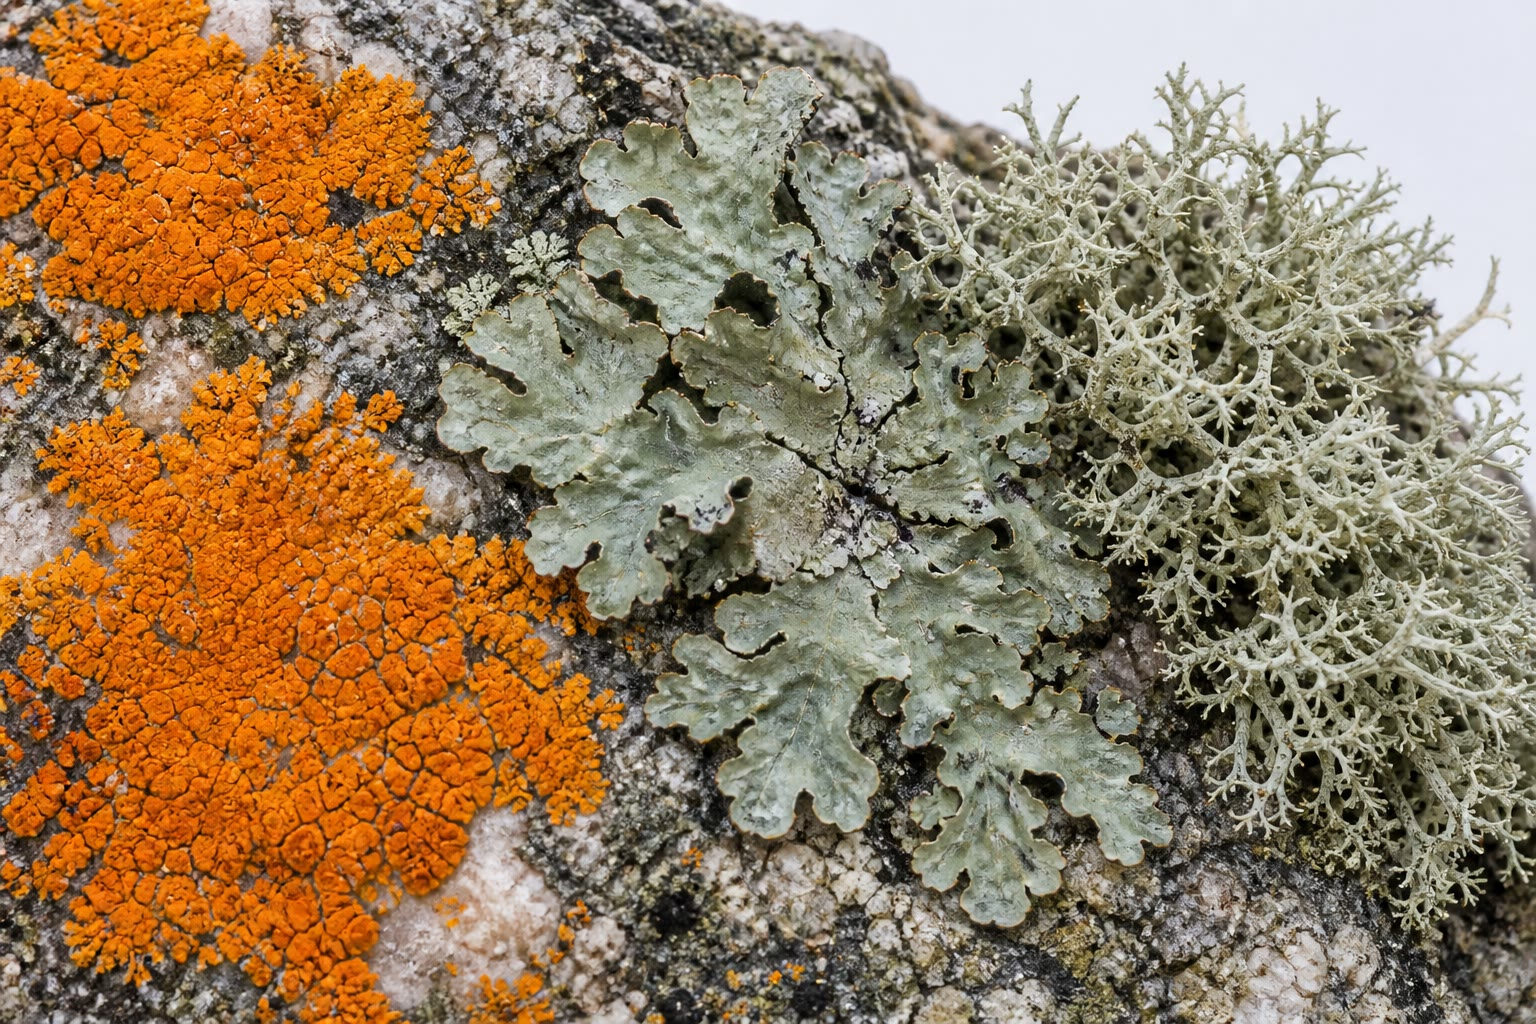
\includegraphics[width=0.46\linewidth]{images/book5/ai/b5-14-lichen.jpg}

{\small Kiri: akar berbintil sebatang kacang, tiap bintil merah mudanya sebuah
pabrik nitrogen berisi bakteroid yang diberi makan gula. Kanan: lumut kerak di
atas batu --- masing-masing sebuah jamur yang merumahkan alga atau sianobakteri
berfotosintesis, yang bersama-sama menjajah permukaan yang tak sanggup
dikuasai satu pun sendirian.}
\end{omfigure}

\section{Kemitraan di laut dan di tempat lain}

\begin{definition}[Karang dan alga]\label{def:b3:microbiomes:coral}
\index{simbiosis karang}\index{zooksantela}\index{pemutihan karang}
Karang pembangun terumbu merumahkan alga dinoflagelata (\emph{Symbiodiniaceae},
yakni \emph{zooksantela}) di dalam sel lapisan ususnya, sejuta atau lebih tiap
sentimeter persegi. Alganya berfotosintesis di dalam jaringan hewannya, dengan
memakai CO$_{2}$, amonia, dan fosfat buangan hewannya, lalu mengembalikan
sampai \qty{90}{\%} karbon yang difiksasinya sebagai gliserol, gula, dan asam
amino, yang memberi makan karangnya dan pengapuran yang membangun terumbunya;
karangnya, pada gilirannya, mengendalikan pasokan nitrogen alganya sehingga
mengendalikan pertumbuhannya. Kemitraan itu bekerja di dalam jendela suhu yang
sempit: ketika airnya bertahan sekitar satu sampai dua derajat di atas maksimum
musim panas selama beberapa minggu, fotosintesis alganya rusak, alganya
melepaskan oksigen reaktif ke dalam sel inangnya, dan karangnya mengusirnya ---
itulah \emph{pemutihan}, dengan rangka putih tembus lewat hewannya yang
bening. Karang yang memutih kelaparan; ia pulih bila airnya mendingin dalam
beberapa minggu dan mati bila tidak. Kekerapan pemutihan telah naik lima kali
lipat sejak tahun 1980, dan itulah mekanisme yang dengannya pemanasan sedang
melenyapkan terumbu.
\end{definition}

\begin{example}[Simbiosis yang membuat habitat]\label{ex:b3:microbiomes:habitats}
Sebuah \emph{lumut kerak} adalah sebuah jamur yang merumahkan alga hijau
atau sianobakteri, dengan jamurnya menyediakan rangka, penahan air, dan mineral yang
terlarut dari batu, dan fotobionnya menyediakan gula (serta, bila sianobakteri,
nitrogen); lumut kerak menutupi sekitar \qty{8}{\%} permukaan darat, menjajah
batu telanjang, lalu memulai pengubahannya menjadi tanah. Cacing tabung
\emph{Riftia} dari lubang laut dalam tidak bermulut maupun berusus ketika
dewasa; ia merumahkan bakteri pengoksidasi sulfida di dalam sebuah trofosom
lalu menghantarkan sulfida dan oksigen kepadanya pada sebuah hemoglobin yang
mengikat keduanya, sambil tumbuh lebih dari semeter setahun di dalam gelap
dengan tenaga kimia. Rayap mencerna kayu dengan sebuah masyarakat usus berisi
protista dan bakteri, dan hewan pemamah biak mencerna rumput dengan sebuah
rumen sebesar bak mandi yang di dalamnya bakteri, arkea, dan jamur meragikan
selulosa menjadi asam lemak dan metana; sapinya hidup dari asam lemak itu dan
dari tubuh mikrobanya sendiri. Pada tiap hal, sebuah kemampuan metabolisme ---
fotosintesis, fiksasi nitrogen, oksidasi sulfida, pencernaan selulosa --- yang
tidak pernah dievolusikan garis keturunan inangnya telah diperoleh lewat
kemitraan dalam satu langkah.
\end{example}

\begin{omfigure}
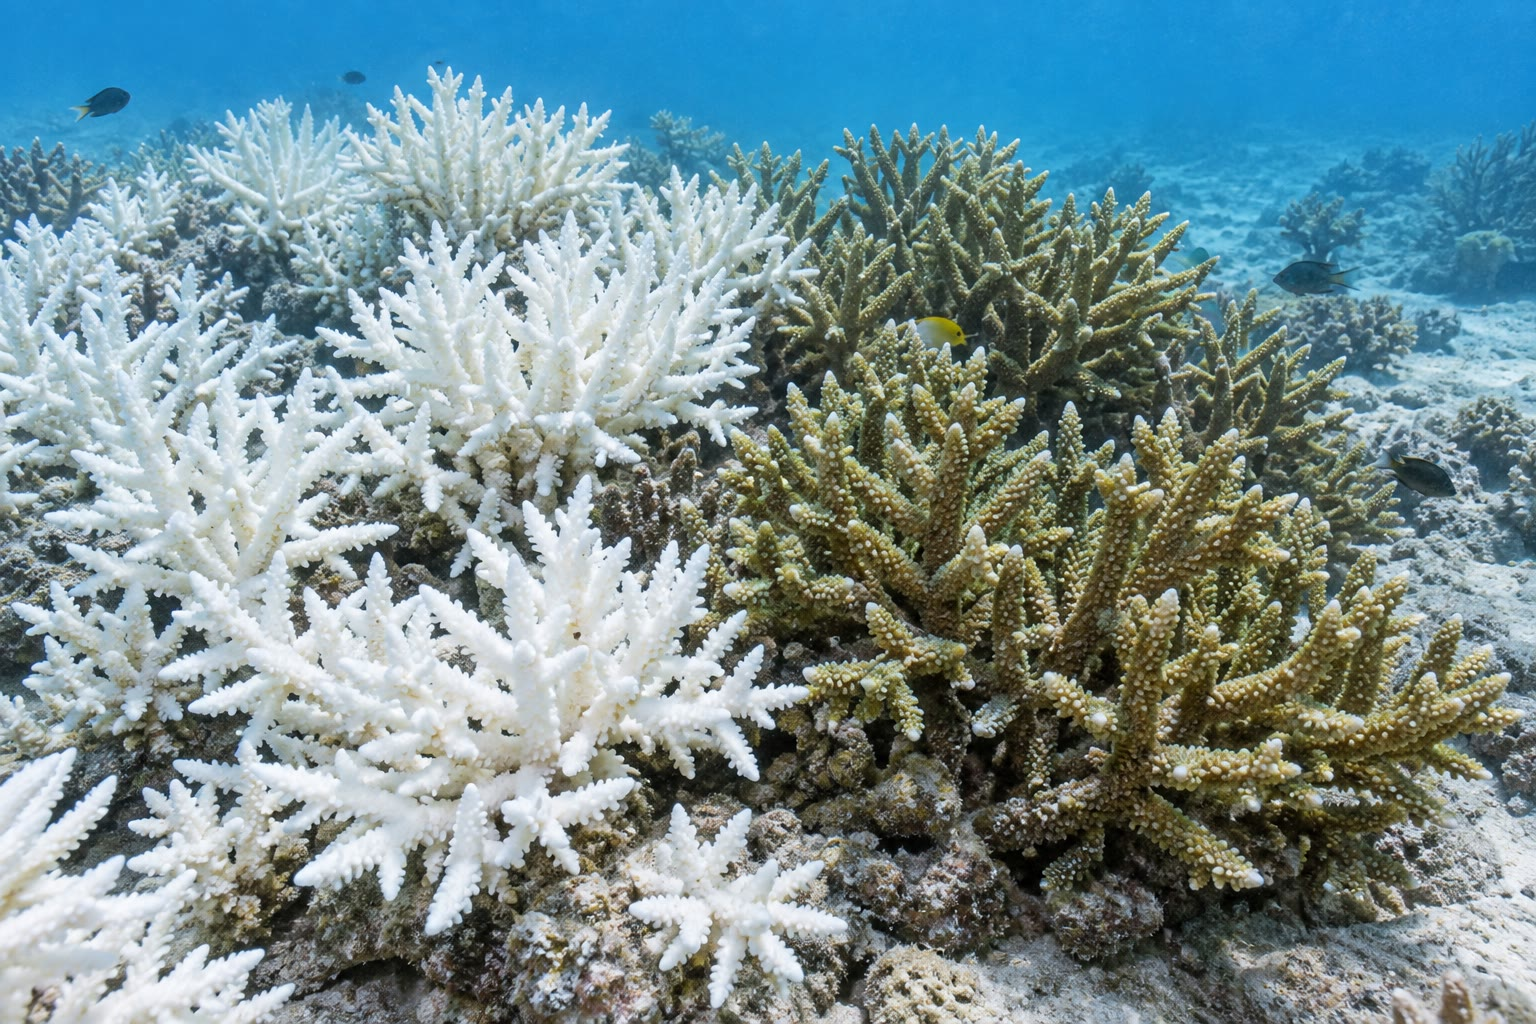
\includegraphics[width=0.56\linewidth]{images/book5/ai/b5-14-coral-bleaching.jpg}

{\small Sebuah terumbu yang separuh memutih: koloni putihnya telah mengusir
alganya sesudah berminggu-minggu air terlalu hangat; yang cokelat masih
menyimpan alganya. Karang putih itu hidup dan kelaparan, dan punya
beberapa minggu untuk dijajahi kembali.}
\end{omfigure}

\begin{omfigure}
\begin{tikzpicture}[every node/.style={font=\scriptsize}, >=stealth]
  % coral cell with alga
  \draw[very thick, omDef, fill=omDef!8] (0,0) ellipse (3.2 and 2.0); \node[above] at (0,2.05) {sel karang (gastroderm)};
  \draw[thick, omMeth!70!black, fill=omMeth!30] (-0.4,-0.1) circle (1.05); \node[align=center] at (-0.4,-0.1) {alga\\(zooksantela)};
  % exchanges
  \draw[->, thick, omMeth!70!black] (0.5,0.4) -- (1.9,0.9) node[right, align=left] {gliserol, gula, asam amino:\\sampai \qty{90}{\%} karbon terfiksasi};
  \draw[<-, thick, omThm] (0.5,-0.5) -- (1.9,-1.0) node[right, align=left] {CO$_2$, NH$_3$, fosfat\\(buangan hewannya)};
  \draw[<-, thick, omProp] (-1.3,0.3) -- (-2.6,1.0) node[left, align=right] {cahaya lewat\\jaringannya};
  \node[below, align=center] at (1.5,-2.1) {tekanan: berminggu-minggu air hangat $\to$ fotosintesis rusak,\\lalu oksigen reaktif $\to$ alga terusir $\to$ pemutihan};
  % thermometer-like bar on the right
  \begin{scope}[xshift=7.6cm, yshift=-1.6cm]
    \draw[thick] (0,0) rectangle (0.5,3.2);
    \fill[omDef!40] (0,0) rectangle (0.5,2.0); \fill[omProp!60] (0,2.0) rectangle (0.5,2.6); \fill[omThm!60] (0,2.6) rectangle (0.5,3.2);
    \node[right] at (0.6,1.0) {jangkauan normal}; \node[right] at (0.6,2.3) {$+\qty{1}{\celsius}$: tekanan}; \node[right, align=left] at (0.6,2.9) {$+\qty{2}{\celsius}$ berminggu-minggu:\\pemutihan};
    \node[below, align=center] at (0.25,-0.1) {suhu laut\\musim panas};
  \end{scope}
\end{tikzpicture}

{\small Pertukaran karang--alga: alganya memfiksasi karbon dengan buangan
hewannya dan cahaya yang lewat jaringannya lalu mengembalikan sebagian besarnya
sebagai makanan; sebuah kenaikan suhu yang kecil dan bertahan memutus kemitraan.}
\end{omfigure}

\section{Dari mitra menjadi organel}

\begin{proposition}[Penyusutan genom dan jalan menuju organel]\label{prop:b3:microbiomes:reduction}
\index{penyusutan genom}\index{pemindahan gen endosimbiotik}
Sebuah endosimbion yang diwarisi lewat telur hidup di dalam populasi beberapa
sel yang tidak pernah berekombinasi dengan pihak luar. Seleksi atasnya lemah
(\cref{ch:b3:molecular-evolution}: populasi kecil memancangkan mutasi yang agak
merugikan lewat hanyutan), gen yang produknya dipasok inangnya tidak
dirindukan ketika rusak, dan gen yang hilang tidak pernah diperoleh kembali.
Genomnya karena itu menyusut, angkatan demi angkatan --- \emph{Buchnera}
menjadi \qty{640}{kb}, sebagian simbion serangga menjadi \qty{140}{kb} dan
beberapa ratus gen, mitokondria menjadi \qty{16}{kb} dan tiga belas protein
pada manusia --- dan inti inangnya memperoleh salinan gen simbionnya
lewat \emph{\omterm{prop:b3:microbiomes:reduction}{pemindahan gen endosimbiotik}}, yang produknya diimpor
kembali dengan sebuah urutan penyasar. Ketika inangnya membuat sebagian besar
protein simbionnya, mengendalikan pembelahannya, dan tidak dapat hidup tanpanya,
simbionnya telah menjadi sebuah organel. Mitokondria dan plastid
menempuh jalan ini dua miliar dan satu miliar tahun lalu
(jilid Tahun~1); kromatofor \emph{Paulinella} adalah pengembara ketiga,
yang telah menempuh seratus juta tahun.
\end{proposition}

\begin{remark}[Perseorangan ditinjau kembali]\label{rem:b3:microbiomes:individual}
Seekor hewan atau sebatang tumbuhan adalah sebuah masyarakat dengan sebuah
genom di pusatnya, yang sebagian besar khazanah metabolismenya, dan banyak
perkembangan serta kekebalannya, bergantung pada mitra yang tidak diwarisinya
di dalam DNA-nya sendiri. Akibat praktisnya sudah ada di sini: \omterm{def:b3:microbiomes:symbiosis}{mikrobiom}
sebagai obat (cangkok tinja), sebagai sasaran obat (kerusakan sampingan
\omterm{def:b3:bacteriology:antibiotics}{antibiotik}, serat makanan sebagai resep), sebagai alat diagnosis, dan sebagai
jalan --- lewat simbion yang direkayasa dan nyamuk pengusung
\emph{Wolbachia} --- untuk mengubah biologi populasi liar. Akibat
teoretisnya adalah bahwa seleksi alam bekerja pada kemitraan, dan
bahwa kemitraan yang terkuat adalah kemitraan yang di dalamnya nasib satu mitra
adalah nasib mitra yang lain.
\end{remark}

\section{Latihan}

\begin{exercise}[$\star$]\label{exo:b3:microbiomes:1}
Definisikanlah \omterm{def:b3:microbiomes:symbiosis}{mutualisme}, \omterm{def:b3:microbiomes:symbiosis}{komensalisme}, dan parasitisme, lalu berilah satu
contoh masing-masing dari bab ini. Mengapa satu pasang spesies dapat berpindah
antarkategori?
\end{exercise}

\begin{exercise}[$\star$]\label{exo:b3:microbiomes:2}
Hitunglah $H$, $e^{H}$, $D$, dan $1/D$ bagi sebuah masyarakat dengan kelimpahan
$0.5$, $0.3$, $0.1$, $0.05$, $0.05$.
\end{exercise}

\begin{exercise}[$\star$]\label{exo:b3:microbiomes:3}
Pertentangkanlah sebuah survei amplikon 16S dengan metagenomika senapan: apa
yang dilaporkan masing-masing, dan apa yang tak dapat dikatakan masing-masing?
\end{exercise}

\begin{exercise}[$\star$]\label{exo:b3:microbiomes:4}
Sebutkanlah empat layanan yang diberikan \omterm{def:b3:microbiomes:gut}{mikrobiom usus} kepada inangnya dan
satu penyakit yang menyusul dari kekacauannya.
\end{exercise}

\begin{exercise}[$\star\star$]\label{exo:b3:microbiomes:5}
Sebuah contoh $N = 20$ \omterm{def:b3:genomics:ngs}{bacaan} memuat spesies dengan $N_{i} = 10, 6, 3, 1$.
Hitunglah $E[S_{n}]$ bagi $n = 5$ dari teoremanya, dan \omterm{thm:b3:microbiomes:rarefaction}{cakupan Good}.
\end{exercise}

\begin{exercise}[$\star\star$]\label{exo:b3:microbiomes:6}
Kolon memuat \qty{400}{g} isi pada $10^{11}$ bakteri per
gram; sebuah bakteri berbobot \qty{1}{pg} dan genomnya bergen \num{4000};
usus seseorang memuat $1000$ spesies. Taksirlah massa
\omterm{def:b3:microbiomes:symbiosis}{mikrobiomnya} dan cacah gen berbedanya, lalu bandingkanlah
dengan \num{20000} milik genom manusia.
\end{exercise}

\begin{exercise}[$\star\star$]\label{exo:b3:microbiomes:7}
Jelaskanlah paradoks oksigen bintil dan bagaimana \omterm{def:b3:microbiomes:nodule}{leghemoglobin} serta
penghadang pembauran menyelesaikannya. Mengapa sebuah bintil berwarna merah
muda, dan apa arti sebuah bintil yang hijau?
\end{exercise}

\begin{exercise}[$\star\star$]\label{exo:b3:microbiomes:8}
Sebuah mutan kacang tidak punya komponen pelonjak kalsium \omterm{def:b3:microbiomes:mycorrhiza}{jalur simbiosis
bersama}. Ramalkanlah pembintilan dan pemikorizaannya, lalu
jelaskanlah apa artinya bagi evolusi kedua \omterm{def:b3:microbiomes:symbiosis}{simbiosis} itu.
\end{exercise}

\begin{exercise}[$\star\star$]\label{exo:b3:microbiomes:9}
Perikanlah percobaan sanksi Kiers dan apa yang akan diramalkan bila
tumbuhannya tidak dapat membedakan bintil yang memfiksasi dari yang tidak.
\end{exercise}

\begin{exercise}[$\star\star\star$]\label{exo:b3:microbiomes:10}
Buktikanlah bahwa $E[S_{n}]$ pada teorema \omterm{def:b3:microbiomes:diversity}{penjarangan} adalah fungsi yang naik
terhadap $n$ lalu mencapai $S$ pada $n = N$, dan tunjukkanlah bahwa bagi sebuah
spesies dengan $N_{i} \ll N$ dan $n \ll N$ peluangnya terlihat kira-kira
$1 - (1 - n/N)^{N_{i}}$.
\end{exercise}

\begin{exercise}[$\star\star\star$]\label{exo:b3:microbiomes:11}
\emph{Wolbachia} ditularkan lewat telur saja. Jelaskanlah mengapa
seleksi atasnya memihak inang betina, perikanlah ketaksesuaian
sitoplasma, lalu tunjukkanlah mengapa hal itu membuat sebuah galur terinfeksi
menyebar walaupun infeksinya berongkos kecil.
\end{exercise}

\begin{exercise}[$\star\star\star$]\label{exo:b3:microbiomes:12}
Dengan memakai \cref{prop:b3:microbiomes:reduction}, jelaskanlah mengapa genom
endosimbion yang ditularkan secara menegak menyusut sedangkan genom kerabatnya
yang hidup bebas tidak, gen mana yang hilang lebih dulu dan mana yang terakhir,
serta apa yang akan membalikkan kecenderungan itu.
\end{exercise}

\section{Soal: Sensus Sebuah Usus}

\begin{problem}[{Soal akhir pekan --- sebuah mikrobiom usus yang dicacah dalam
sel, gen, dan kalori, keanekaannya diukur dan dijarangkan, anggaran nitrogen
sebatang kacang diimbangkan terhadap gulanya, serta karbon sebuah terumbu
dihitung, berakhir pada kalori yang diperoleh sebuah mikrobiom, cakupan
sebuah contoh pengurutan, dan gula yang dibayar sepetak kacang bagi
nitrogennya}]
\label{pb:b3:microbiomes:1}
Data: isi kolon \qty{400}{g} pada $10^{11}$ bakteri per gram, dengan massa
sel \qty{1}{pg}; $1000$ spesies, \num{4000} gen masing-masing, \qty{30}{\%}
gennya dibagi antara dua spesies mana pun. Makanan: \qty{30}{g} serat tiap
hari, yang diragikan menjadi \omterm{def:b3:microbiomes:gut}{asam lemak rantai pendek} pada \qty{10}{mmol} tiap gram,
masing-masing bernilai \qty{0.9}{kJ}; makanan sebesar \qty{9000}{kJ}. Sebuah contoh pengurutan:
$N = 2000$ \omterm{def:b3:genomics:ngs}{bacaan}, $S = 180$ spesies, $f_{1} = 60$ tunggalan; kelimpahan
ketiga spesies teratas $0.30$, $0.20$, $0.10$, sisanya tersebar rata.
Sepetak kacang memfiksasi \qty{150}{kg} N tiap hektare tiap musim lalu membayar
\qty{8}{g} gula tiap gram N yang difiksasi; fotosintesisnya menghasilkan
\qty{12}{t} gula tiap hektare tiap musim. \omterm{def:b3:microbiomes:nodule}{Nitrogenase}: $16$ ATP tiap
N$_{2}$. Sebuah karang: $10^{6}$ alga tiap cm$^{2}$, masing-masing memfiksasi \qty{20}{pg}
karbon sehari, \qty{90}{\%} diteruskan ke inangnya; jaringan karangnya
bernapas \qty{15}{\micro g} karbon tiap cm$^{2}$ tiap hari.

\medskip
\noindent\textbf{Bagian I --- Sel dan gen.}
\begin{enumerate}
  \item Berapa banyak bakteri di dalam kolon, dan berapa bobotnya?
  \item Setara berapa banyak genom bakteri DNA itu, dan bagaimana
        totalnya dibandingkan dengan DNA di dalam $3\times 10^{13}$ sel
        manusia (masing-masing \qty{6.4}{pg})?
  \item Taksirlah cacah gen bakteri yang berbeda di dalam ususnya,
        dengan memperhitungkan tindihan \qty{30}{\%} (cacahlah \qty{70}{\%}
        tiap spesies yang tak terbagi ditambah satu himpunan bersama).
        Bandingkanlah dengan \num{20000}.
  \item Berapa milimol \omterm{def:b3:microbiomes:gut}{asam lemak rantai pendek} yang dihasilkan seratnya
        tiap hari, berapa kilojoule, dan berapa bagian dari
        makanannya?
  \item Seekor mencit bebas kuman memerlukan \qty{30}{\%} lebih banyak makanan.
        Cukupkah sumbangan asam lemak pada pertanyaan 4 untuk menjelaskannya?
        Apa lagi yang mungkin?
  \item Bakteri membelah di dalam kolon kira-kira sekali sehari dan isinya
        dibuang pada laju yang sama. Keadaan mantap apa yang diisyaratkannya,
        dan apa yang terjadi pada masyarakatnya ketika sekali pengobatan
        \omterm{def:b3:bacteriology:antibiotics}{antibiotik} membunuh \qty{99.9}{\%} selnya?
\end{enumerate}

\medskip
\noindent\textbf{Bagian II --- Keanekaan.}
\begin{enumerate}[resume]
  \item Hitunglah kelimpahan nisbi tiap dari $177$ spesies
        kecilnya, lalu \omterm{def:b3:microbiomes:diversity}{indeks Shannon} $H$ dan $e^{H}$.
  \item Hitunglah \omterm{def:b3:microbiomes:diversity}{indeks Simpson} $D$ dan $1/D$. Mengapa $1/D$ lebih kecil
        daripada $e^{H}$?
  \item \omterm{thm:b3:microbiomes:rarefaction}{Cakupan Good} contohnya; berapa \omterm{def:b3:genomics:ngs}{bacaan} tiap seribu yang tergolong
        spesies yang belum terlihat?
  \item Sebuah contoh kedua sebesar \num{10000} \omterm{def:b3:genomics:ngs}{bacaan} dari usus yang sama
        menghasilkan $260$ spesies. Jelaskanlah, dengan memakai teorema
        \omterm{def:b3:microbiomes:diversity}{penjarangan}, mengapa ini bukan pertentangan, dan apa yang harus
        dilakukan sebelum membandingkan keduanya.
  \item Pada teoremanya, berapa peluang bahwa sebuah spesies dengan
        $N_{i} = 1$ muncul di dalam anak contoh $n = 1000$ dari $N =
        2000$? Dengan $N_{i} = 5$?
  \item Sesudah \omterm{def:b3:bacteriology:antibiotics}{antibiotik} usus yang sama menunjukkan $60$ spesies, $H = 2.0$,
        dan satu spesies pada kelimpahan $0.5$. Hitunglah $e^{H}$ dan $D$ lalu
        perikanlah masyarakatnya dengan kata-kata.
\end{enumerate}

\medskip
\noindent\textbf{Bagian III --- Neraca bintil.}
\begin{enumerate}[resume]
  \item Berapa banyak gula yang dibayar tanamannya tiap hektare bagi
        \qty{150}{kg} N-nya, dan berapa bagian fotosintesisnya
        yang demikian?
  \item Berapa mol N$_{2}$ kah \qty{150}{kg} N itu, dan berapa
        mol ATP yang dibelanjakan \omterm{def:b3:microbiomes:nodule}{nitrogenase} atasnya?
  \item Pada $30$ ATP tiap glukosa yang dinapaskan, berapa kilogram glukosa
        yang diwakili ATP itu? Bandingkanlah dengan gula yang dibayar; untuk
        apa sisanya?
  \item Amonia industri berongkos sekitar \qty{35}{MJ} tiap kg N. Dengan
        memakai \qty{16}{kJ} tiap gram gula, bandingkanlah ongkos tenaga
        nitrogen tanamannya dengan ongkos pabriknya.
  \item Sebuah rizobium yang tidak memfiksasi memasuki sebuah bintil. Bila
        tumbuhannya menjatuhkan sanksi dengan memotong separuh oksigennya, dan
        perkembangbiakannya turun separuh, berapa bagian \omterm{def:b3:microbiomes:nodule}{rizobia} musim
        berikutnya yang berupa pencurang bila mereka mulai pada \qty{10}{\%}
        dan pemfiksasinya berkembang biak normal? (Satu putaran.)
  \item Tanpa sanksi, pencurang yang menghemat ongkos memfiksasi
        berkembang biak \qty{20}{\%} lebih banyak. Selama sepuluh musim, berapa
        bagiannya yang berupa pencurang, dari awal yang sama? Apa yang
        ditunjukkan perbandingan itu?
\end{enumerate}

\medskip
\noindent\textbf{Bagian IV --- Neraca terumbu.}
\begin{enumerate}[resume]
  \item Berapa banyak karbon yang difiksasi alga satu sentimeter persegi tiap
        hari, dan berapa banyak yang sampai ke karangnya?
  \item Bandingkanlah dengan pernapasan karangnya. Berapa lebihnya, dan
        untuk apa lebihnya dipakai?
  \item Sesudah pemutihan, \qty{95}{\%} alganya lenyap. Hitunglah ulang
        karbon yang dipasoknya. Berapa lama karangnya dapat bertahan pada
        cadangan \qty{300}{\micro g} karbon tiap cm$^{2}$?
  \item Tekanannya kerap diukur dalam minggu-derajat-panas: jumlah,
        sepanjang musimnya, kelebihan mingguan di atas maksimum musim
        panasnya. Delapan minggu pada $+\qty{1}{\celsius}$ atau empat pada
        $+\qty{2}{\celsius}$ sama-sama memberi $8$; pemutihan mulai dekat $4$.
        Mana di antara kedua tampang itu yang lebih buruk, dan mengapa
        ukurannya toh mungkin berhasil?
  \item Karang dapat merumahkan beberapa spesies alga dengan batas suhu yang
        berbeda. Usulkanlah bagaimana sebuah terumbu mungkin menyesuaikan diri,
        dan apa yang membatasinya.
  \item Sebuah terumbu seluas \qty{1}{km^2} permukaan karang hidup: berapa
        banyak karbon yang difiksasi alganya tiap hari dan tiap tahun, dalam ton?
  \item Ringkaslah: bagian makanan yang dipasok \omterm{def:b3:microbiomes:symbiosis}{mikrobiomnya}
        (pertanyaan~4), cakupan contoh pengurutannya
        (pertanyaan~9), dan bagian fotosintesis yang dibayar sepetak kacang
        bagi nitrogennya (pertanyaan~13).
\end{enumerate}
\end{problem}
